\documentclass[../main.tex]{subfiles}

\graphicspath{../images/}

\begin{document}

\section{Vector Analysis}
\barh 

\paragraph{1.1}
\begin{figure}[ht]
    \centering
    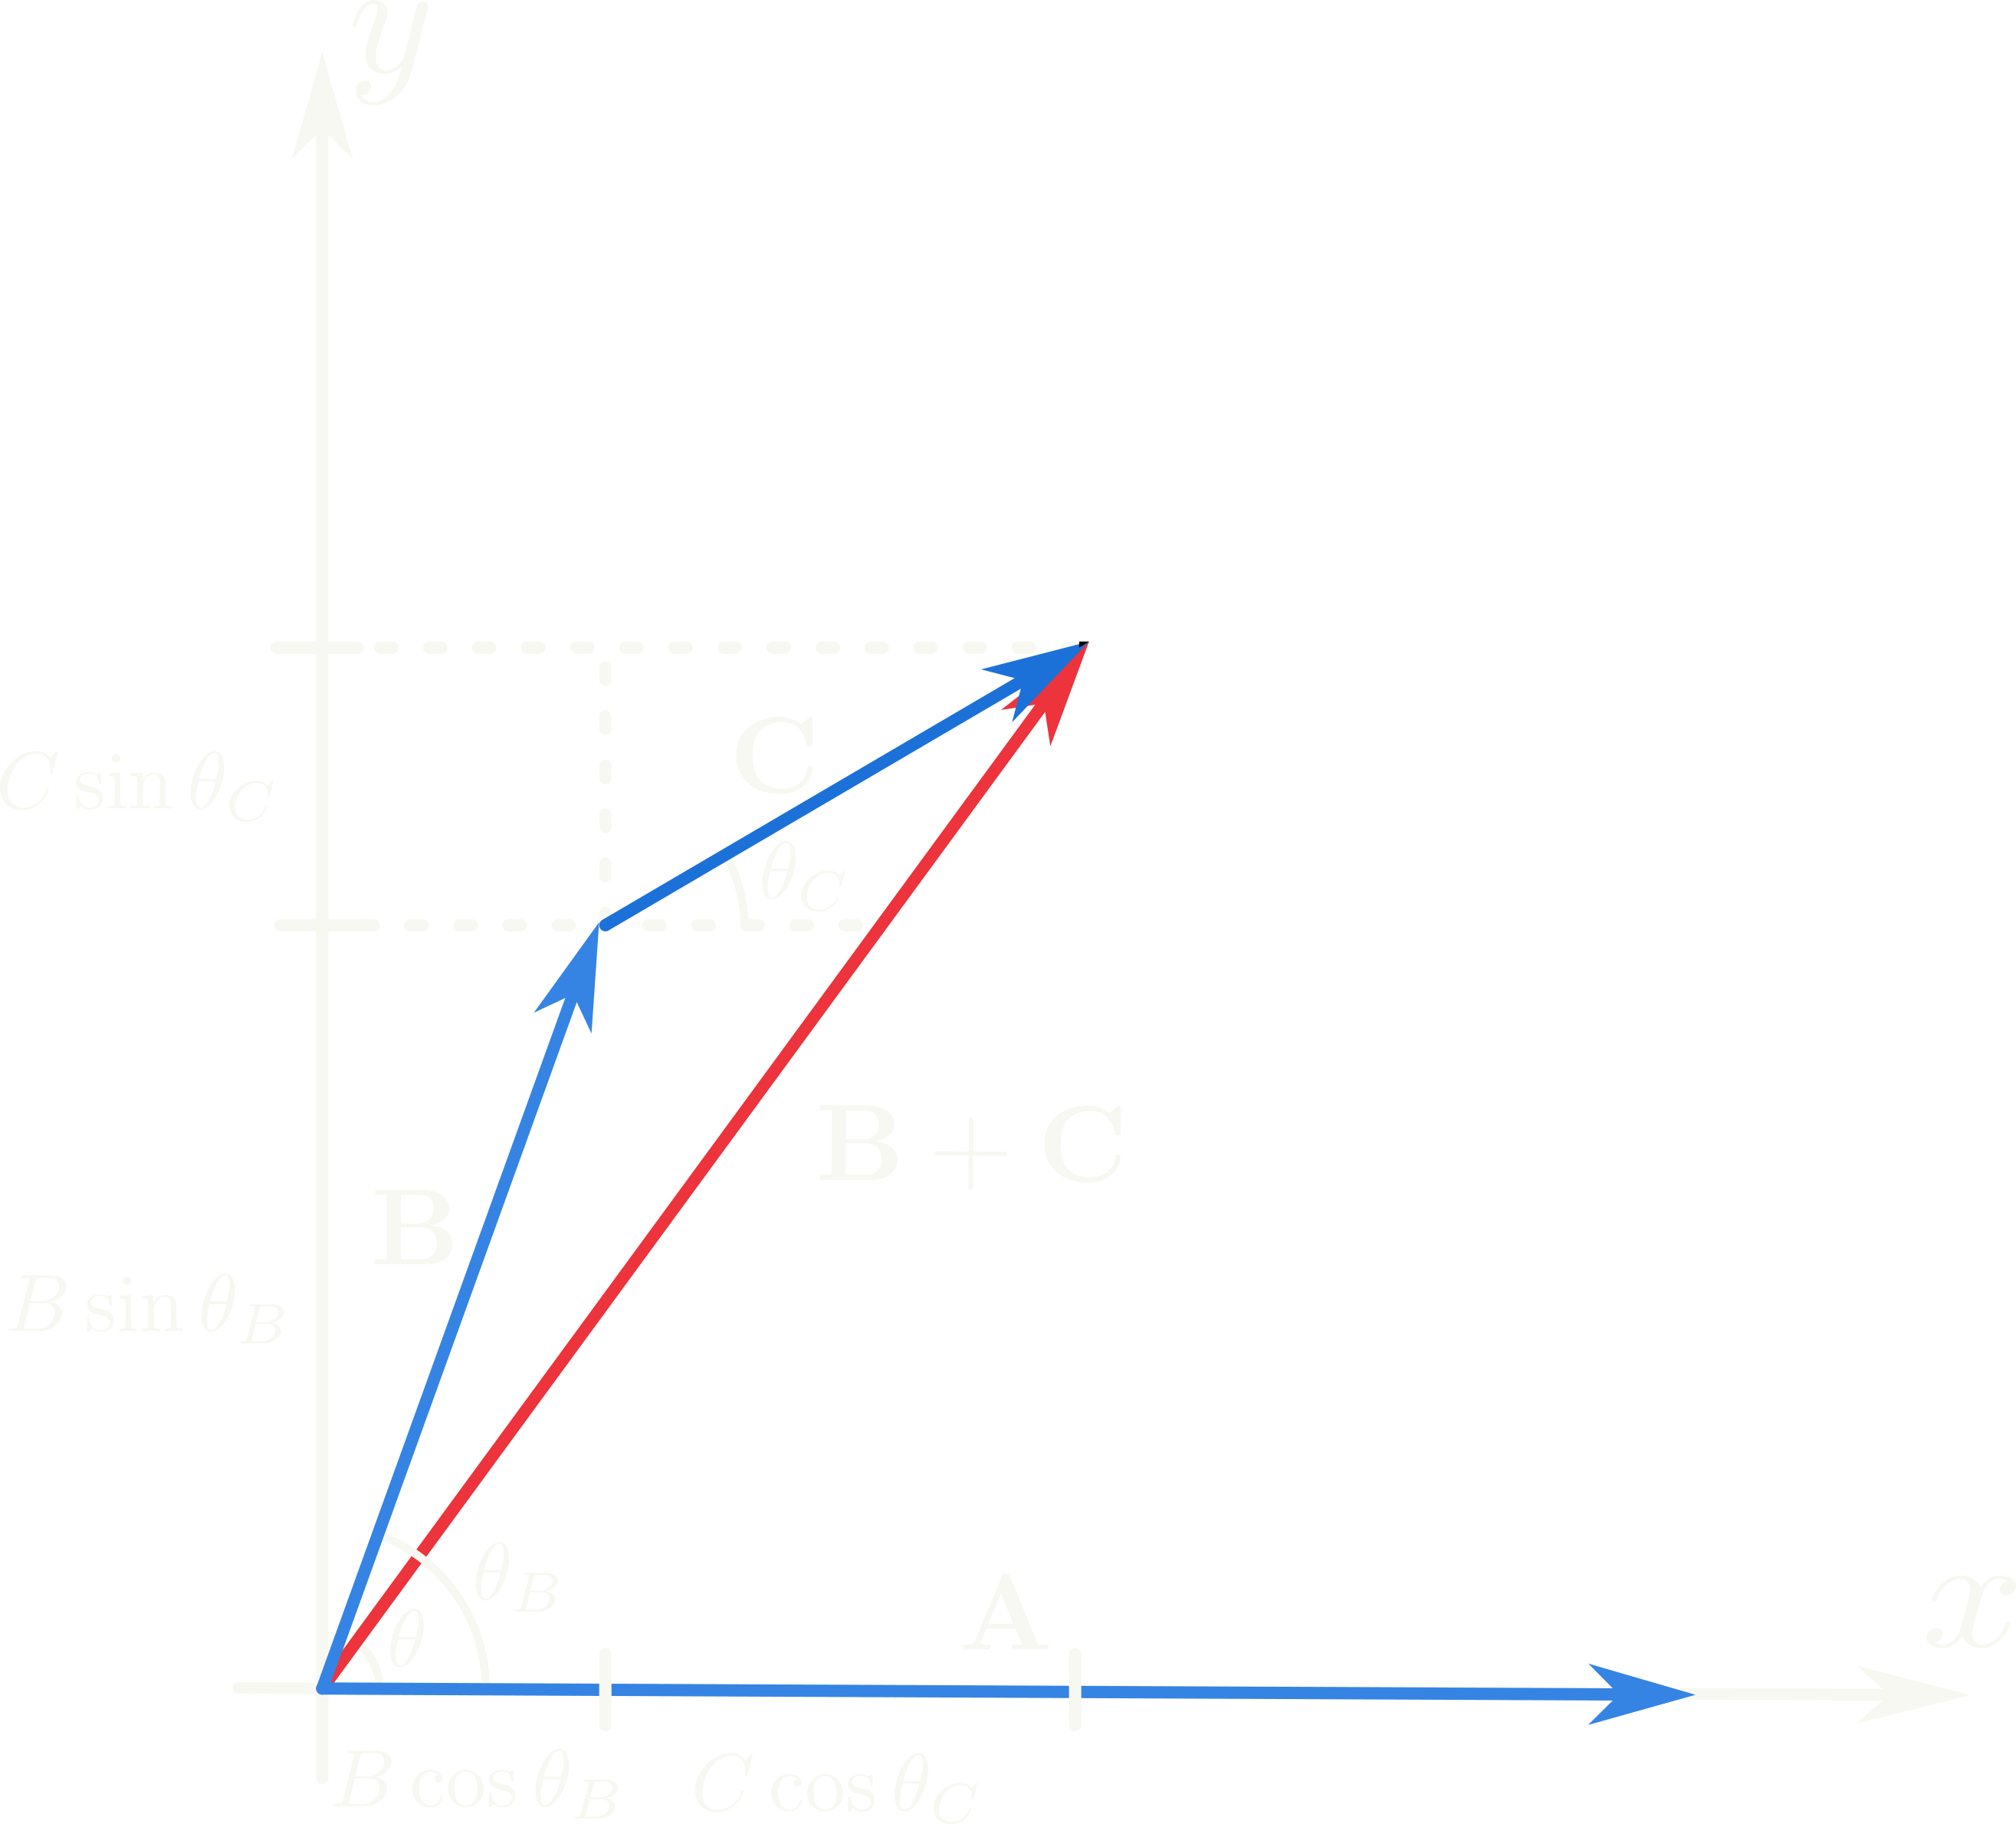
\includegraphics[width=0.5\linewidth]{images/fig1_1.png}
    \caption{Three Coplanar Vectors}
    \label{fig:1.1}
\end{figure}
(a) When three vectors are coplanar as shown in Figure \ref{fig:1.1}, the dot product is
\begin{align*}
    \vb{A} \cdot (\vb{B} + \vb{C}) &= \vb{A} \cdot \vb{B} + \vb{A} \cdot \vb{C} \\
    A (B+C) \cos \theta &= A B \cos \theta_B + A C \cos \theta_C
\end{align*}
Since $B \cos{\theta_B} + B \cos{\theta_C} = (B+C)\cos{\theta}$ from Figure \ref{fig:1.1}, the
distriubtive property holds true. The cross product also holds true since
$B \sin{\theta_B} + B \sin{\theta_C} = (B+C)\sin{\theta}$, and multiplying by $A$ on both sides
gives the same result as the distriubtive property:
\begin{align*}
    \vb{A} \cp (\vb{B} + \vb{C}) &= \vb{A} \cp\vb{B} + \vb{A} \cp\vb{C} \\
    A (B+C) \sin \theta &= A B \sin \theta_B + A C \sin \theta_C
\end{align*}

(b) In the general case in three-dimensional space, each vector has three components: \\
$\vb{A} = (A_x, A_y, A_z)$. Therefore,
\begin{align*}
    \vb{A} \cdot (\vb{B} + \vb{C}) &=
        \vb{A} \cdot (B_x + C_x, B_y + C_y, B_z + C_z) \\
    &= A_x (B_x + C_x) + A_y (B_y + C_y) + A_z (B_z + C_z) \\
    &= A_x B_x + A_y B_y + A_z B_z + A_x C_x + A_y C_y + A_z C_z \\
    &= \vb{A} \cdot \vb{B} + \vb{A} \cdot \vb{C}
\end{align*}

\paragraph{1.2}
Setting $\vb{A} = \vb{B} = (1, 1, 1)$ and $\vb{C} = (1, 1, -1)$:
\begin{align*}
    (\vb{A} \cp \vb{B}) \cp \vb{C} &\overset{?}{=} \vb{A} \cp (\vb{B} \cp \vb{C})\\
    0 &\overset{?}{=} (1, 1, 1) \cp [(1, 1, 1) \cp (1, 1, -1)]\\
    0 &\overset{?}{=} (1, 1, 1) \cp (-2, 2, 0)\\
    0 &\neq (-2, -2, 4)
\end{align*}
where the cross product of parallel vectors $\vb{A} \cp \vb{B} = 0$. Therefore, the cross product is
not associative.

\paragraph{1.3}
Taking the dot product of a unit cube's body diagonals $\vb{A} = (1, 1, 1)$, $\vb{B} = (1, 1, -1)$:
\begin{align*}
    \vb{A} \cdot \vb{B} &= AB \cos{\theta} \\
    1 &= 3 \cos{\theta} \\
    \theta &= \arccos{1/3} \approx \ang{70.53}
\end{align*} 

\paragraph{1.4}
The cross product of two vectors coplanar to the shaded plane---$\vb{A} = (-1, 2, 0)$,
$\vb{B} = (-1, 0, 3)$---is parallel to the normal unit vector $\vu{n}$ of the plane:
\begin{align*}
    \vb{A} \cp \vb{B} &= \vb{C} \\
    \begin{vmatrix}
        \vu{x} & \vu{y} & \vu{z} \\
        -1 & 2 & 0 \\
        -1 & 0 & 3
    \end{vmatrix} &= (6, 3, 2) \\
\end{align*}
where $\vu{n} = \vb{C} / C$, and $C = \sqrt{6^2 + 3^2 + 2^2} = \sqrt{49} = 7$. Therefore,
\begin{align*}
    \vu{n} &= \frac{1}{7} (6, 3, 2)
\end{align*}

\paragraph{1.5}
Proving the ``BAC--CAB'' rule for three-dimensional vectors:
\begin{align*}
    \vb{A} \cp (\vb{B} \cp \vb{C}) &= \vb{A} \cp
    \begin{vmatrix}
        \vu{x} & \vu{y} & \vu{z} \\
        B_x & B_y & B_z \\
        C_x & C_y & C_z
    \end{vmatrix} \\
    &= \begin{vmatrix}
        \vu{x} & \vu{y} & \vu{z} \\
        A_x & A_y & A_z \\
        B_y C_z - B_z C_y & B_z C_x - B_x C_z & B_x C_y - B_y C_x
    \end{vmatrix}
\end{align*}
where the $x$ component is $A_y (B_x C_y - B_y C_x) - A_z (B_z C_x - B_x C_z)$. Similarly,
\begin{align*}
    \vb{B}(\vb{A} \cdot \vb{C}) - \vb{C}(\vb{A} \cdot \vb{B}) &=
        \vb{B} (A_x C_x + A_y C_y + A_z C_z) - \vb{C} (A_x B_x + A_y B_y + A_z B_z)
\end{align*}
where $x$ component simplifes to
\begin{align*}
    B_x (\cancel{A_x C_x} + A_y C_y + A_z C_z) - C_x (\cancel{A_x B_x}+ A_y B_y + A_z B_z) &=
        A_y (B_x C_y - B_y C_x) - A_z (B_z C_x - B_x C_z)
\end{align*}
the same is done for the $y$ and $z$ components. Therefore, the ``BAC--CAB'' rule holds true.

\paragraph{1.6}
\begin{align*}
    [\vb{A} \cp (\vb{B} \cp \vb{C})] + [\vb{B} \cp (\vb{C} \cp \vb{A})] 
        + [\vb{C} \cp (\vb{A} \cp \vb{B})]
    &= \cancel{\vb{B}(\vb{A} \cdot \vb{C})} - \vb{C}(\vb{A} \cdot \vb{B})
    + \vb{C}(\vb{B} \cdot \vb{A}) = 0 \\ &- \vb{A}(\vb{B} \cdot \vb{C})
    + \vb{A}(\vb{C} \cdot \vb{B}) - \cancel{\vb{B}(\vb{C} \cdot \vb{A})}\\
\end{align*}
since dot product is associative, the first and last terms cancel out, and the middle terms also
cancel out with each other.

\begin{align*}
    \vb{A} \cp (\vb{B} \cp \vb{C}) &= (\vb{A} \cp \vb{B}) \cp \vb{C} \\
    \vb{B} (\vb{A} \cdot \vb{C}) - \vb{C} (\vb{A} \cdot \vb{B}) &=
    \vb{B} (\vb{A} \cdot \vb{C}) - \vb{A} (\vb{B} \cdot \vb{C}) \\
    0 &= -\vb{C} (\vb{A} \cdot \vb{B}) + \vb{A} (\vb{B} \cdot \vb{C}) \\
    0 &= -\vb{B} (\vb{C} \cp \vb{A}) = (\vb{C} \cp \vb{A}) \cp \vb{B}
\end{align*}
For the relation to hold true, either the vectors $\vb{A}$ and $\vb{C}$  are parallel
($\vb{A} \cp \vb{A} = 0$) or $\vb{B}$ is perpendicular to both $\vb{A}$ and $\vb{C}$
($\vb{A} \cdot \vb{B} = \vb{B} \cdot \vb{C} = 0$).

\paragraph{1.7}
Finding the seperation vector $\boldscriptr$:
\begin{align*}
    \boldscriptr &= \vb{r} - \vb{r}' = (4, 6, 8) - (2, 8, 7) = (2, -2, 1) \\
    \scriptr &= \sqrt{2^2 + (-2)^2 + 1^2} = 3 \\
    \vu{\boldscriptr} &= \quantity(\frac{2}{3}, -\frac{2}{3}, \frac{1}{3})
\end{align*}

\paragraph{1.8} (a)
\begin{align*}
    \begin{split}
        \bar{A}_y \bar{B}_y + \bar{A}_z \bar{B}_z =
        (A_y \cos{\phi} &+ A_z \sin{\phi})(B_y \cos{\phi} + B_z \sin{\phi}) \\
        &+ (-A_y \sin\phi + A_z \cos\phi)(-B_y \sin\phi + B_z \cos\phi)
    \end{split} \\
    \begin{split}
        = A_y B_y \cos^2\phi + A_z B_z \sin^2\phi
        &+ \cancel{A_y B_z \sin\phi\cos\phi} + \bcancel{A_z B_y \sin\phi\cos\phi} \\
        + A_y B_y \sin^2\phi &- \cancel{A_y B_z \sin\phi\cos\phi} 
        - \bcancel{A_z B_y \sin\phi\cos\phi} + A_z B_z \cos^2\phi
    \end{split} \\
    = A_y B_y (\sin^2\phi + \cos^2\phi) &+ A_z B_z (\sin^2\phi + \cos^2\phi) \\
    \bar{A}_y \bar{B}_y + \bar{A}_z \bar{B}_z &= A_y B_y + A_z B_z
\end{align*}
(b) To preserve length $\abs{\bar{A}} = \abs{A}$. Squaring both sides and expanding gives
\begin{align*}
    \bar{A}_x^2 + \bar{A}_y^2 + \bar{A}_z^2 = A_x^2 + A_y^2 + A_z^2
\end{align*}
in summation form,
\begin{align*}
    \sum_{i=1}^3 \bar{A}_i \bar{A}_i
    = \sum_{i=1}^3 \quantity(\sum_{j=1}^3 R_{ij} A_j) \quantity(\sum_{k=1}^3 R_{ik} A_k)
    = \sum_{i=1}^3 \sum_{j=1}^3 \sum_{k=1}^3 R_{ij} R_{ik} A_j A_k
\end{align*}
For the length to be preserved, the indices $j$ and $k$ must be equal. Therefore,
\begin{align*}
    R_{ij} R_{ik} = \delta_{jk}
\end{align*}
where $\delta_{ij}$ is the Kronecker delta. Thus the length is preserved if the rotation
matrix is orthogonal, i.e.
\begin{align*}
    R_{ij} R_{ik} = (R^T)_{ji} R_{ik} = \delta_{jk} \qor R^T R = I
\end{align*}

\paragraph{1.9}
\begin{figure}[ht]
    \centering
    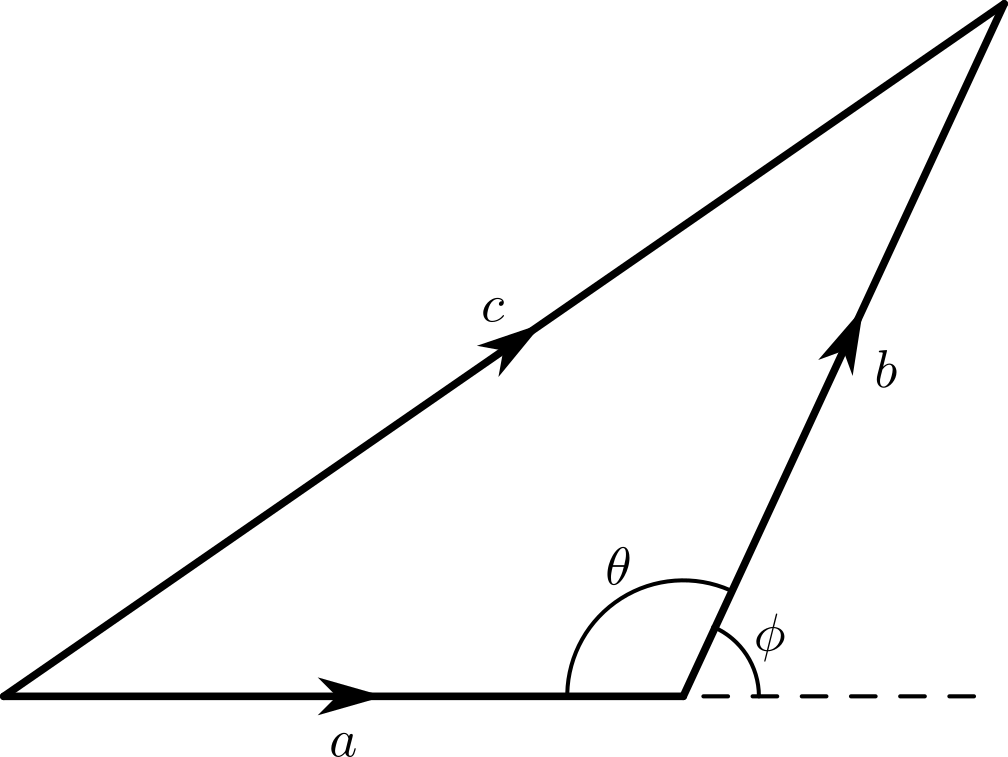
\includegraphics[width=0.4\linewidth]{images/fig1_9.png}
    \caption{Rotation of $\ang{120}$ about an axis through the origin and point $(1, 1, 1)$}
    \label{fig:1.9}
\end{figure}
From Figure \ref{fig:1.9}, the rotation is equivalent to changing the position of the basis vectors
$\vu{x} \to \vu{z}$, $\vu{y} \to \vu{x}$, and $\vu{z} \to \vu{y}$. Therefore, the rotation matrix is
a permutation matrix:
\begin{align*}
    R = \begin{pmatrix}
        0 & 0 & 1 \\
        1 & 0 & 0 \\
        0 & 1 & 0
    \end{pmatrix}
\end{align*}

\paragraph{1.10}
(a) Under a \textbf{translation} of coordinates $\bar{y} = y - a$, the origin $O$ and terminus
$A = (x, y, z)$ of some vector are translated to
\begin{align*}
    O \to O' &= (0, -a, 0)\\
    A \to A' &= (x, y - a, z)
\end{align*}
therefore, the translated vector is
\begin{align*}
    \overline{O'A'} &= (x, y - a, z) - (0, -a, 0) = (x, y, z) = \overline{OA} = \vb{A}
\end{align*}
which is the same as the original vector, so
\begin{align*}
    \mqty(\bar{A}_x \\ \bar{A}_y \\ \bar{A}_z) &=  \mqty(A_x \\ A_y \\ A_z)
\end{align*}

(b) Under \textbf{inversion} of coordinates, only the terminus changes
\begin{align*}
    O \to O' &= (0, 0, 0) \\
    A \to A' &= (-x, -y, -z)
\end{align*}
therefore, the inverted vector is
\begin{align*}
    \overline{O'A'} = (-x, -y, -z) \qor \mqty(\bar{A}_x \\ \bar{A}_y \\ \bar{A}_z) &=
        \mqty(-A_x \\ -A_y \\ -A_z)
\end{align*}

(c) The components of cross product under inversion
\begin{align*}
    \bar{\vb{A}} \cross \bar{\vb{B}} &= 
    \begin{pmatrix}
        \bar{A}_y \bar{B}_z - \bar{A}_z \bar{B}_y \\
        \bar{A}_z \bar{B}_x - \bar{A}_x \bar{B}_z \\
        \bar{A}_x \bar{B}_y - \bar{A}_y \bar{B}_x
    \end{pmatrix}
    =
    \begin{pmatrix}
        A_y B_z - A_z B_y \\
        A_z B_x - A_x B_z \\
        A_x B_y - A_y B_x
    \end{pmatrix}
\end{align*}
which is the same as the original cross product $\vb{A} \cross \vb{B}$. The cross product of two
pseudovectors is also a pseudovector. Torque $\vb{\tau} = \vb{r} \cross \vb{F}$ and magnetic force
$\vb{F} = q \vb{v} \cross \vb{B}$ are examples of pseudovectors.

(d) Scalar triple product under inversion
\begin{align*}
    \bar{A} \cdot (\bar{B} \cross \bar{C}) &= -\vb{A} \cdot (-\vb{B} \cross -\vb{C}) \\
    &= -\vb{A} \cdot (\vb{B} \cross \vb{C})
\end{align*}
the scalar triple product changes sign under inversion.

\paragraph{1.11}
(a) Finding gradient of $f(x, y, z) = x^2 + y^3 + z^4$:
\begin{align*}
    \grad{f} &= \pdv{f}{x} \vu{x} + \pdv{f}{y} \vu{y} + \pdv{f}{z} \vu{z} \\
    &= 2x \vu{x} + 3y^2 \vu{y} + 4z^3 \vu{z}
\end{align*}
(b) Gradient of $f(x, y, z) = x^2y^3z^4$:
\begin{align*}
    \grad{f} = 2xy^3z^4 \vu{x} + 3x^2y^2z^4 \vu{y} + 4x^2y^3z^3 \vu{z}
\end{align*}
(c) Gradient of $f(x, y, z) = e^x \sin(y) \ln(z)$:
\begin{align*}
    \grad{f} = e^x \vu{x} + e^x \cos(y) \ln(z) \vu{y} + \frac{e^x \sin(y)}{z} \vu{z}
\end{align*}

\paragraph{1.12}
The height of the hill (in feet) is given by the function
\begin{align*}
    h(x, y) = 10 (2xy - 3x^2 - 4y^2 - 18x + 28y + 12)
\end{align*}
where $y$ is north and $x$ is east in miles. The gradient of $h$ is
\begin{align*}
    \grad{h} &= 10 (2y - 6x - 18) \vu{x} + 10 (2x - 8y + 28) \vu{y}
\end{align*}
(a) The top of the hill is a stationary point, so the summit is found by setting the gradient to
zero which gives the system of equations
\begin{align*}
    0 &= 2y - 6x - 18 & 0 &= 2x - 8y + 28
\end{align*}
adding the first equation to 3 times the second equation gives
\begin{align*}
    0 &= 2y - 6x - 18 + 3(2x - 8y + 28) \\
    0 &= -22y + 66 \\
    y &= 3
\end{align*}
substituting $y = 3$ into the first equation
\begin{align*}
    0 = 2(3) - 6x - 18 \to x = -2
\end{align*}
Therefore, the top of the hill is at $(-2, 3)$ or 2 miles west and 3 miles north of the origin.

(b) The height of the hill is simply $h(-2, 3) = 10(12) = 720$ feet.

(c) The steepness of the hill at $h(1,1)$ is given by the magnitude of the gradient
\begin{align*}
    \abs{\grad{h}} &= 10\sqrt{(2y - 6x - 18)^2 + (2x - 8y + 28)^2} \\
    &= 10\sqrt{(2 - 6 - 18)^2 + (2 - 8 + 28)^2} \\
    &= 10\sqrt{(-22)^2 + (22)^2} = 220 \sqrt{2} \approx \qty{311}{ft/mi}
\end{align*}
The direction of the steepest slope is given by the vector in the direction of the gradient
at the point $\grad{h(1,1)} = 220(-\vb{x} + \vb{y})$, or simply northwest.

\paragraph{1.13}
Given the seperation vector
\begin{align*}
    \boldscriptr = (x - x') \vu{x} + (y - y') \vu{y} + (z - z') \vu{z} \qand 
    \scriptr = \sqrt{(x - x')^2 + (y - y')^2 + (z - z')^2}
\end{align*}
(a) Show that $\grad(\scriptr^2) = 2 \boldscriptr$:
\begin{align*}
    \grad(\scriptr^2) = 2(x - x') \vu{x} + 2(y - y') \vu{y} + 2(z - z') \vu{z} = 2 \boldscriptr
\end{align*}

(b)
\begin{align*}
    \grad(\frac{1}{\scriptr}) &= \pdv{x}(\frac{1}{\scriptr}) \vu{x}
        + \pdv{y}(\frac{1}{\scriptr}) \vu{y} + \pdv{z}(\frac{1}{\scriptr}) \vu{z} \\
\end{align*}
looking at the $x$ component,
\begin{align*}
    \pdv{x}(\frac{1}{\scriptr}) &= -\frac{1}{\scriptr^2} \pdv{x}(\scriptr) \\
    &= -\frac{1}{\scriptr^2} \pdv{x}(\sqrt{(x - x')^2 + (y - y')^2 + (z - z')^2}) \\
    &= -\frac{1}{\scriptr^2} \frac{1}{2}
        \frac{2(x - x')}{\sqrt{(x - x')^2 + (y - y')^2 + (z - z')^2}} \\
    &= -\frac{x - x'}{\scriptr^3}
\end{align*}
therefore,
\begin{align*}
    \grad(\frac{1}{\scriptr}) = -\frac{1}{\scriptr^3}
        [(x - x') \vu{x} + (y - y') \vu{y} + (z - z') \vu{z}]
    = -\frac{\boldscriptr}{\scriptr^3} 
    = -\frac{\vu{\boldscriptr}}{\scriptr^2}
\end{align*}

(c) The general formula is
\begin{align*}
    \grad(\scriptr^n) = n \scriptr^{n-1} \vu{\boldscriptr}
\end{align*}

\paragraph{1.14}
Given the rotation matrix
\begin{align*}
    \mqty(\bar{y} \\ \bar{z}) &= \mqty(\cos\phi & \sin\phi \\ -\sin\phi & \cos\phi)
    \mqty(y \\ z)
\end{align*}
or the two equations
\begin{align*}
    \bar{y} &= y \cos\phi + z \sin\phi \\
    \bar{z} &= -y \sin\phi + z \cos\phi
\end{align*}
differentiating with respect to $\bar{y}$ and $\bar{z}$ respectively gives
\begin{align*}
    1 &= \pdv{y}{\bar{y}}\cos\phi + \pdv{z}{\bar{y}}\sin\phi \\
    1 &= -\pdv{y}{\bar{z}}\sin\phi + \pdv{z}{\bar{z}}\cos\phi
\end{align*}
this can only be true if
\begin{align*}
    \pdv{y}{\bar{y}} = \cos\phi     ,\quad      \pdv{z}{\bar{y}} = \sin\phi
    \qand \pdv{y}{\bar{z}} = -\sin\phi      ,       \pdv{z}{\bar{z}} = \cos\phi
\end{align*}
which satisfies the trig identity $\sin^2\phi + \cos^2\phi = 1$. Differentiating $f$ with respect to
the rotated coordinates $\bar{y}$ and $\bar{z}$ is given by
\begin{align*}
    \pdv{f}{\bar{y}} &= \pdv{f}{y} \pdv{y}{\bar{y}} + \pdv{f}{z} \pdv{z}{\bar{y}}
    = \pdv{f}{y} \cos\phi + \pdv{f}{z} \sin\phi \\
    \pdv{f}{\bar{z}} &= \pdv{f}{y} \pdv{y}{\bar{z}} + \pdv{f}{z} \pdv{z}{\bar{z}}
    = -\pdv{f}{y} \sin\phi + \pdv{f}{z} \cos\phi
\end{align*}
therefore, the gradient of $f$ transforms as a vector under rotations given by
\begin{align*}
    \overline{\grad{f}} = \pdv{f}{\bar{y}} \vu{\bar{y}} + \pdv{f}{\bar{z}} \vu{\bar{z}}
    = \quantity(\pdv{f}{y} \cos\phi + \pdv{f}{z} \sin\phi) \vu{\bar{y}}
    + \quantity(-\pdv{f}{y} \sin\phi + \pdv{f}{z} \cos\phi) \vu{\bar{z}}
\end{align*}
or in matrix form
\begin{align*}
    \overline{\grad{f}} = \mqty(\cos\phi & -\sin\phi \\ \sin\phi & \cos\phi) \grad{f}
\end{align*}
where the gradient is a column vector
\begin{align*}
    \grad{f} = \begin{pmatrix}
        \pdv{f}{y} \\[1ex] \pdv{f}{z}
    \end{pmatrix}
\end{align*}

\paragraph{1.15}
(a) Calculating divergence of $v_a = x^2\vu{x} + 3xz^2\vu{y} - 2xz\vu{z}$:
\begin{align*}
    \div{v_a} &= \pdv{v_{ax}}{x} + \pdv{v_{ay}}{y} + \pdv{v_{az}}{z} \\
    &= 2x + 0 - 2x = 0
\end{align*}

(b) $v_b = xy\vu{x} + 2yz\vu{y} + 3zx\vu{z}$:
\begin{align*}
    \div{v_b} &= y + 2z + 3x
\end{align*}

(c) $v_c = y^2\vu{x} + (2xy + z^2)\vu{y} + 2yz\vu{z}$:
\begin{align*}
    \div{v_c} &= 0 + 2x + 2y = 2(x + y)
\end{align*}

\paragraph{1.16}
\begin{figure}[ht]
    \centering
    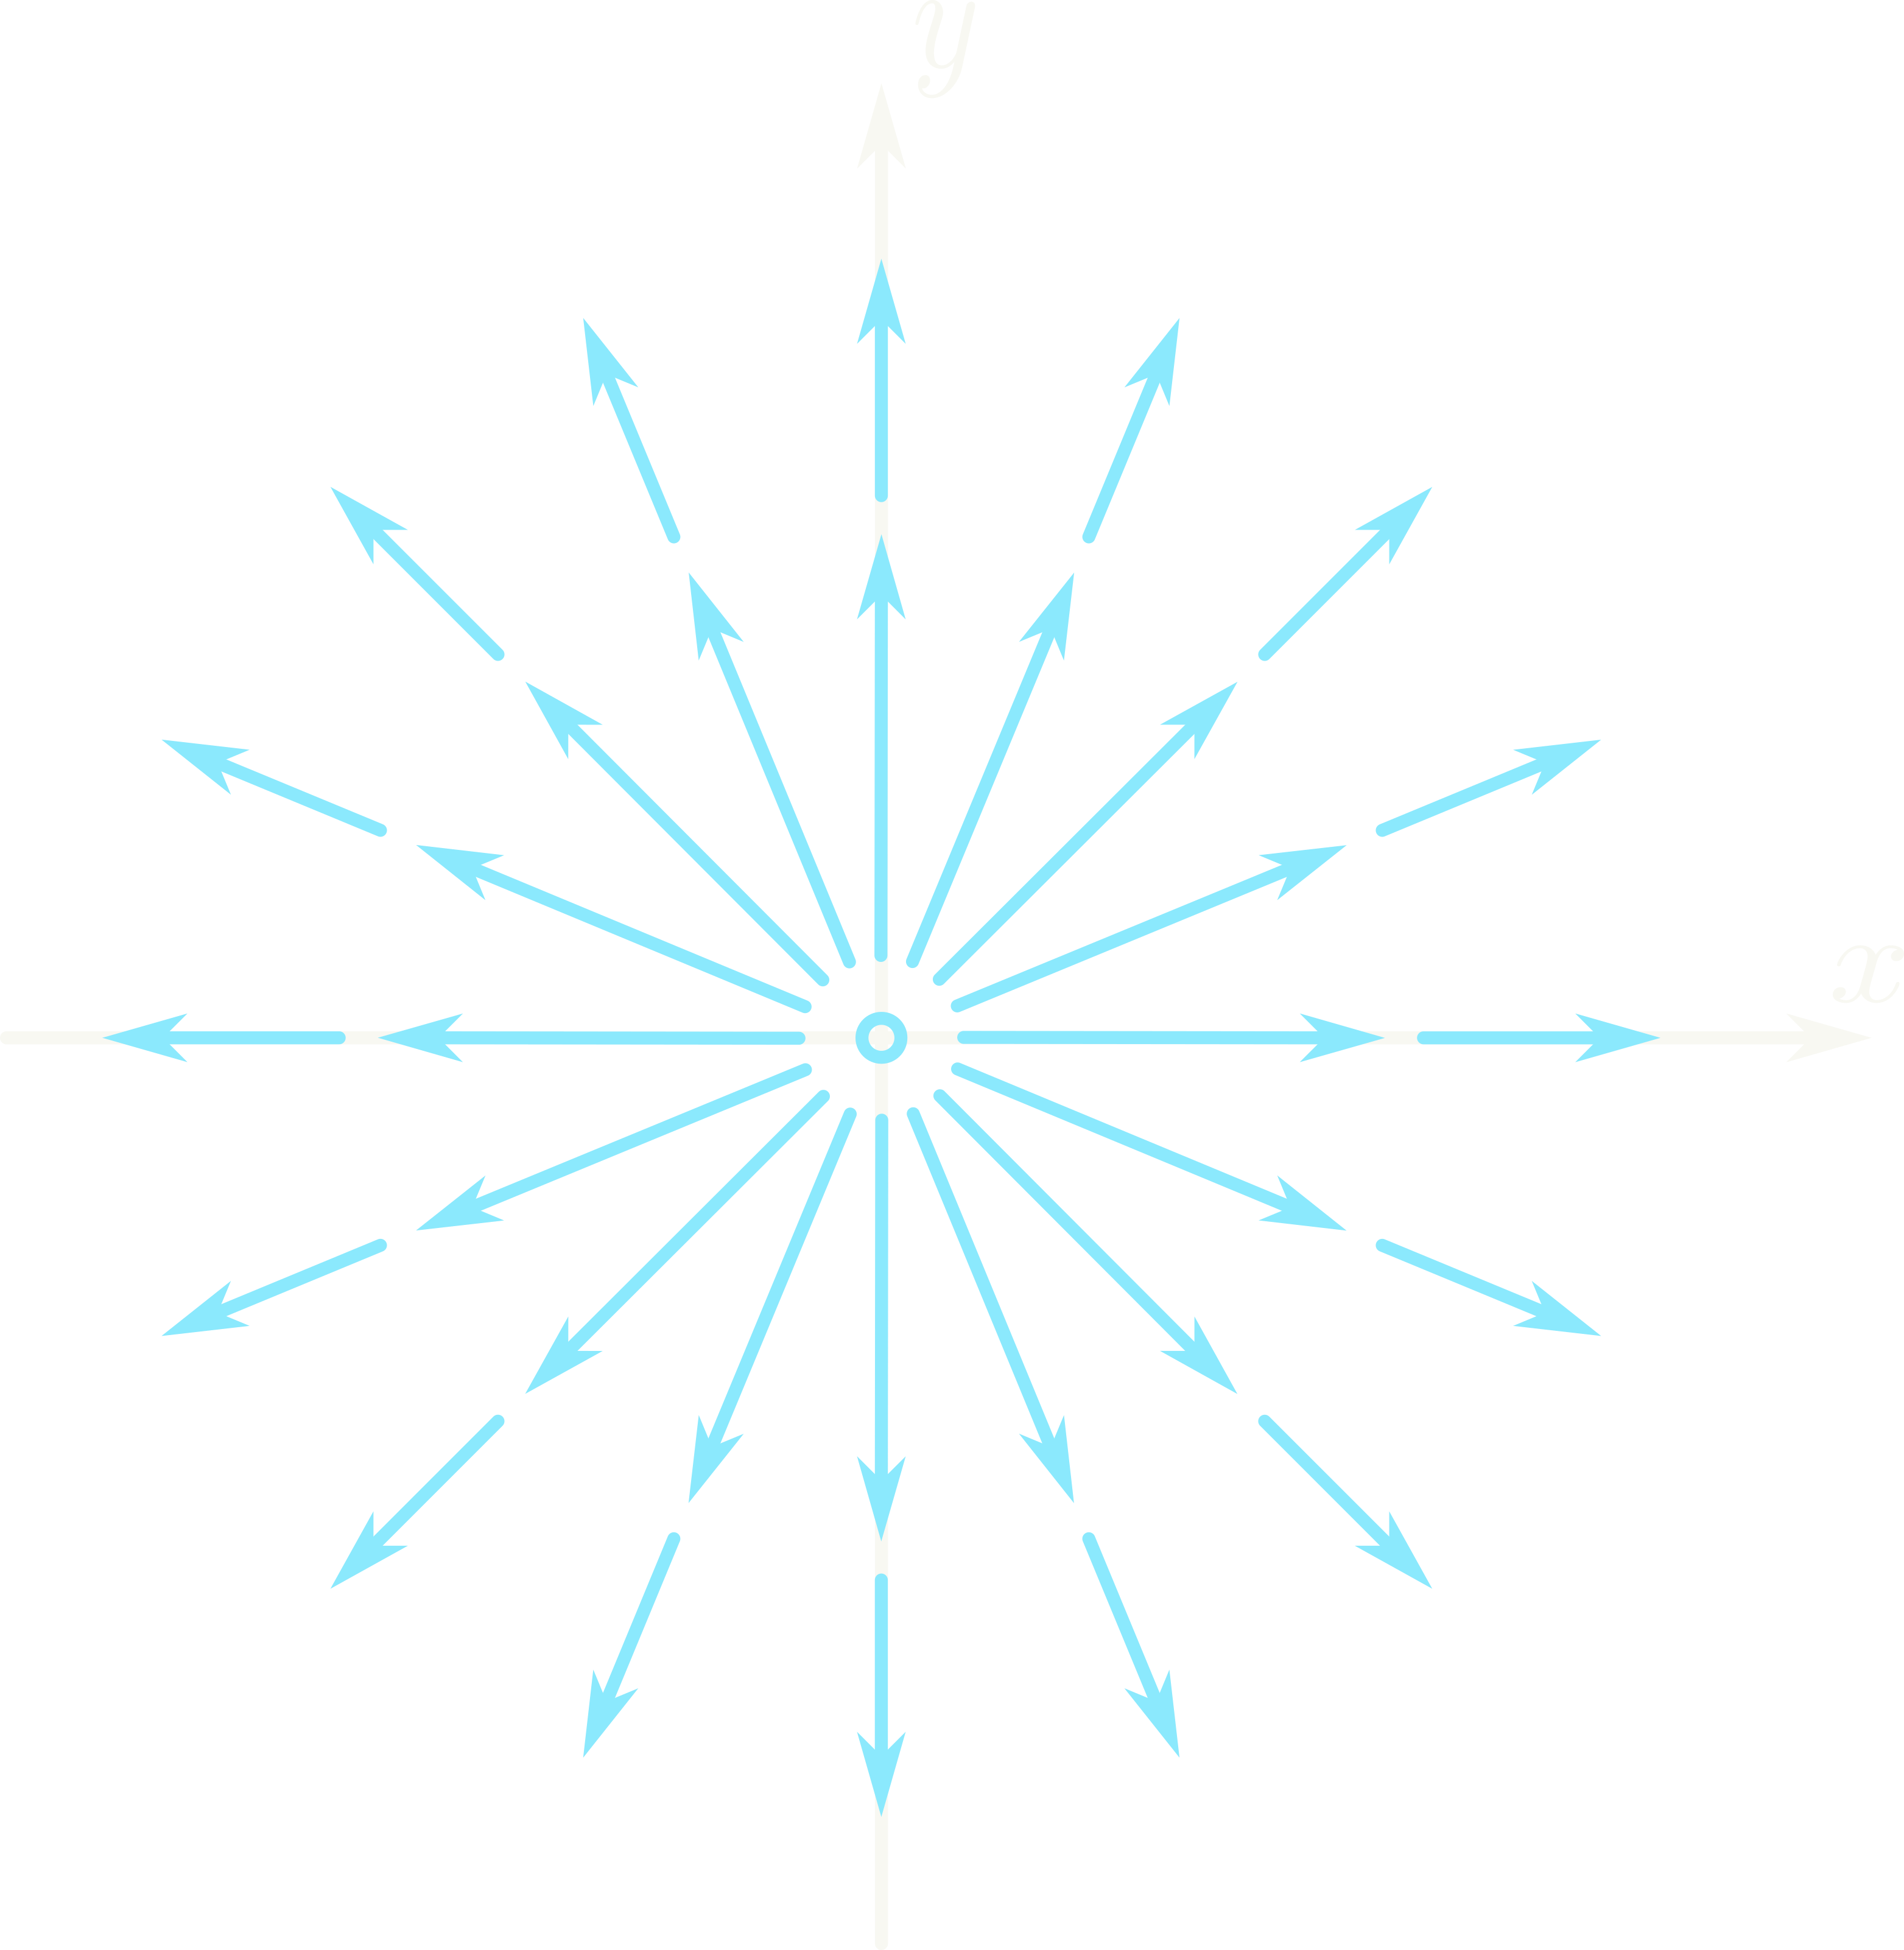
\includegraphics[width=0.4\linewidth]{images/fig1_16.png}
    \caption{Sketch of the vector field $\vb{v} = \vu{r} / r^2$}
    \label{fig:1.16}
\end{figure}
Given
\begin{align*}
    r = \sqrt{x^2 + y^2 + z^2} \qand
    \vu{r} = \frac{\vb{r}}{r} = \frac{x\vu{x} + y\vu{y} + z\vu{z}}{\sqrt{x^2 + y^2 + z^2}}
\end{align*}
where $\vb{r} = x\vu{x} + y\vu{y} + z\vu{z}$ is the position vector. The vector functions is
\begin{align*}
    v = \frac{\vu{r}}{r^2} = \frac{\vb{r}}{r^3}
\end{align*}
where the components are
\begin{align*}
    v_x = \frac{x}{r^3} \qand v_y = \frac{y}{r^3} \qand v_z = \frac{z}{r^3}
\end{align*}
Looking at the $x$ component of the divergence,
\begin{align*}
    [\div{\vb{v}}]_x &= \pdv{v_x}{x} \\
    &= \pdv{x}(\frac{x}{r^3}) \\
    &= \pdv{x}(\frac{x}{(x^2 + y^2 + z^2)^{3/2}}) \qq{using chain rule...}\\
    &= \frac{1}{(x^2 + y^2 + z^2)^{3/2}} - \frac{3x^2}{(x^2 + y^2 + z^2)^{5/2}} \\
    &= \frac{1}{r^3} - \frac{3x^2}{r^5}
\end{align*}
therefore, the divergence of $\vb{v}$ is
\begin{align*}
    \div{\vb{v}} &= \quantity(\frac{1}{r^3} - \frac{3x^2}{r^5})
        + \quantity(\frac{1}{r^3} - \frac{3y^2}{r^5})
        + \quantity(\frac{1}{r^3} - \frac{3z^2}{r^5}) \\
    &= \frac{3}{r^3} - 3\frac{x^2 + y^2 + z^2}{r^5} \\
    &= \frac{3}{r^3} - 3\frac{r^2}{r^5} = 0
\end{align*}
This is consistent with the sketch in Figure \ref{fig:1.16} because the vector field is not `sourcing' or
`sinking'.

\paragraph{1.17}
Given
\begin{align*}
    \bar{v}_y = v_y \cos\phi + v_z \sin\phi \qand \bar{v}_z = -v_y \sin\phi + v_z \cos\phi
\end{align*}
Calculating the derivatives
\begin{align*}
    \pdv{\bar{v}_y}{\bar{y}} &= \pdv{v_y}{\bar{y}} \cos\phi + \pdv{v_z}{\bar{y}} \sin\phi \\
    \pdv{\bar{v}_z}{\bar{z}} &= -\pdv{v_y}{\bar{z}} \sin\phi + \pdv{v_z}{\bar{z}} \cos\phi
\end{align*}
from Problem 1.14,
\begin{align*}
    \pdv{f}{\bar{y}} &= \pdv{f}{y} \cos\phi + \pdv{f}{z} \sin\phi \\
    \pdv{f}{\bar{z}} &= -\pdv{f}{y} \sin\phi + \pdv{f}{z} \cos\phi
\end{align*}
therefore, the derivatives are rewritten as
\begin{align*}
    \pdv{\bar{v}_y}{\bar{y}} &=
        \quantity(\pdv{v_y}{y} \pdv{y}{\bar{y}} + \pdv{v_y}{z} \pdv{z}{\bar{y}}) \cos\phi 
        + \quantity(\pdv{v_z}{y} \pdv{y}{\bar{z}} + \pdv{v_z}{y} \pdv{z}{\bar{z}}) \sin\phi \\
    &= \quantity(\pdv{v_y}{y} \cos\phi + \pdv{v_y}{z} \sin\phi) \cos\phi 
        + \quantity(\pdv{v_z}{y} \cos\phi + \pdv{v_z}{z} \sin\phi) \sin\phi
\end{align*}
and likewise,
\begin{align*}
    \pdv{\bar{v}_z}{\bar{z}} &=
        - \quantity(-\pdv{v_y}{y} \sin\phi +\pdv{v_y}{z} \cos\phi) \sin\phi 
        + \quantity(-\pdv{v_z}{y} \sin\phi + \pdv{v_z}{z} \cos\phi) \cos\phi \\
\end{align*}
Finally adding the two equations together gives
\begin{align*}
    \div{\bar{\vb{v}}} &= \pdv{\bar{v}_y}{\bar{y}} + \pdv{\bar{v}_z}{\bar{z}} \\
    &= \pdv{v_y}{y} \cos^2\phi + \pdv{v_y}{z} \sin\phi\cos\phi 
        + \pdv{v_z}{y} \sin\phi\cos\phi + \pdv{v_z}{z} \sin\phi^2 \\
    &+ \pdv{v_y}{y} \sin^2\phi - \pdv{v_y}{z} \sin\phi\cos\phi
        - \pdv{v_z}{y} \sin\phi\cos\phi + \pdv{v_z}{z} \cos^2\phi \\
    &= (\sin\phi^2 + \cos\phi^2)\quantity[\pdv{v_y}{y} + \pdv{v_z}{z}] \\
    &= \pdv{v_y}{y} + \pdv{v_z}{z}
\end{align*}
which shows that the divergence transforms as a scalar under rotations.

\paragraph{1.18}
Curl of vector functions from Problem 1.15:
(a) $\vb{v}_a = x^2\vu{x} + 3xz^2\vu{y} - 2xz\vu{z}$:
\begin{align*}
    \curl{\vb{v}_a} &= \mqty|
        \vu{x} & \vu{y} & \vu{z} \\
        \pdv{x} & \pdv{y} & \pdv{z} \\
        x^2 & 3xz^2 & -2xz
    | \\
    &= \vu{x} (0 - 6xz) - \vu{y} (-2z - 0) + \vu{z} (3z^2 - 0) \\
    &= -6xz\vu{x} + 2z\vu{y} + 3z^2\vu{z}
\end{align*}

(b) $\vb{v}_b = xy\vu{x} + 2yz\vu{y} + 3zx\vu{z}$:
\begin{align*}
    \curl{\vb{v}_b} &= \begin{vmatrix}
        \vu{x} & \vu{y} & \vu{z} \\
        \pdv{x} & \pdv{y} & \pdv{z} \\
        xy & 2yz & 3zx
    \end{vmatrix} \\
    &= \vu{x} (0 - 2y) - \vu{y} (3z - 0) + \vu{z} (0 - x) \\
    &= -2y\vu{x} - 3z\vu{y} - x\vu{z}
\end{align*}

(c) $\vb{v}_c = y^2\vu{x} + (2xy + z^2)\vu{y} + 2yz\vu{z}$:
\begin{align*}
    \curl{\vb{v}_c} &= \begin{vmatrix}
        \vu{x} & \vu{y} & \vu{z} \\
        \pdv{x} & \pdv{y} & \pdv{z} \\
        y^2 & 2xy + z^2 & 2yz
    \end{vmatrix} \\
    &= \vu{x} (2z - 2z) - \vu{y} (0 - 0) + \vu{z} (2y - 2y) \\
    &= 0
\end{align*}

\paragraph{1.19}
\begin{figure}[ht]
    \centering
    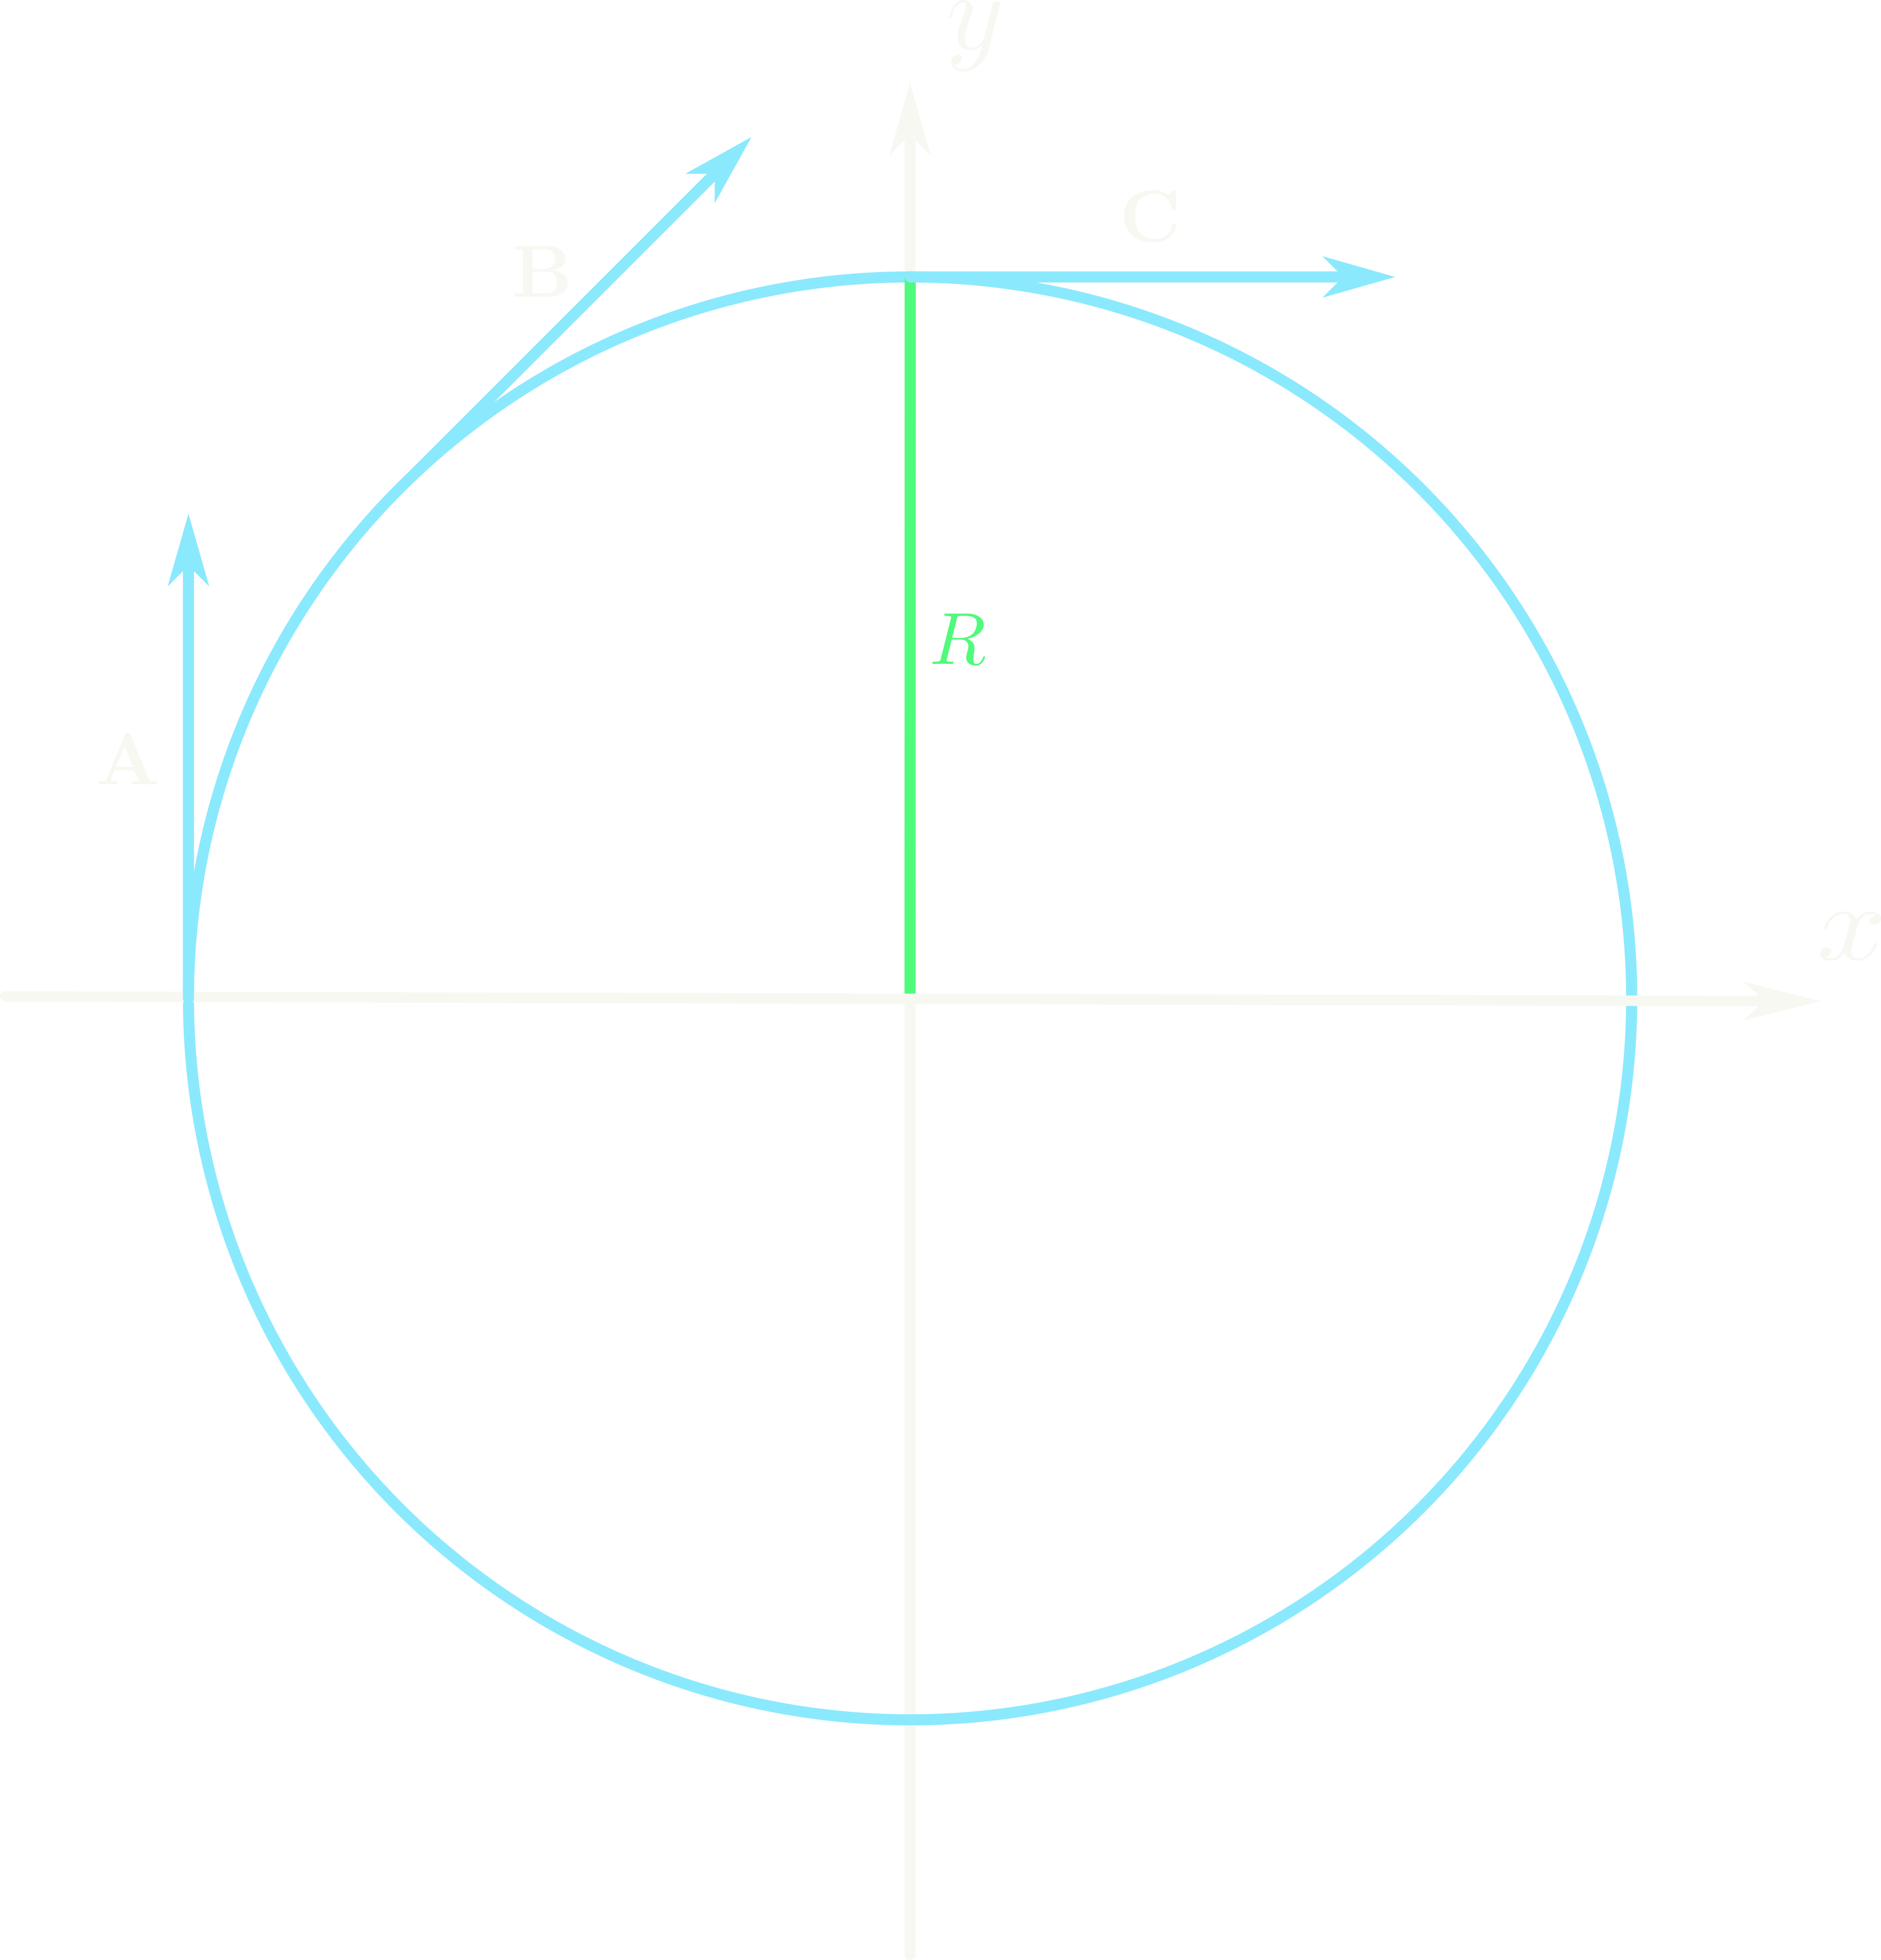
\includegraphics[width=0.4\linewidth]{images/fig1_19.png}
    \caption{Sketch of the vector field pointing clockwise around a circle of radius $R$}
    \label{fig:1.19}
\end{figure}
From Figure \ref{fig:1.19}, the sign of $\pdv*{v_x}{y}$ is positive, and the sign of $\pdv*{v_y}{x}$
is negative. Therefore, the curl
\begin{align*}
    \curl{\vb{v}} = \vu{z} \quantity(\pdv{v_x}{y} - \pdv{v_y}{z}) 
\end{align*}
is in the negative $z$ direction, or into the page. This is consistent with the right-hand rule as
the thumb points into the page.

\paragraph{1.20}
Proof that the vector function
\begin{align*}
    \vb{g} = \frac{\vu{r}}{r^2} = \frac{\vb{r}}{r^3} = \frac{x\vu{x} + y\vu{y} + z\vu{z}}{r^3}
\end{align*}
has zero divergence and curl given
\begin{align*}
    \pdv{r}{x_i} = \frac{x_i}{r} \qand \pdv{x}{y} = \frac{y}{x} = 0
\end{align*}
From Problem 1.16, the divergence of $\vb{g}$ is
\begin{align*}
    \div{\vb{g}} &= \pdv{g_x}{x} + \pdv{g_y}{y} + \pdv{g_z}{z} \\
    &= \pdv{x}(\frac{x}{r^3}) + \pdv{y}(\frac{y}{r^3}) + \pdv{z}(\frac{z}{r^3}) \\
    &= \frac{1}{r^3} - \frac{3x^2}{r^5} + \frac{1}{r^3} - \frac{3y^2}{r^5}
        + \frac{1}{r^3} - \frac{3z^2}{r^5} \\
    &= \frac{3}{r^3} - \frac{3}{r^3} = 0
\end{align*}
and the curl is
\begin{align*}
    \curl{\vb{g}} &= \begin{vmatrix}
        \vu{x} & \vu{y} & \vu{z} \\
        \pdv{x} & \pdv{y} & \pdv{z} \\
        \frac{x}{r^3} & \frac{y}{r^3} & \frac{z}{r^3}
    \end{vmatrix} \\
    &= \vu{x} (0 - 0) - \vu{y} (0 - 0) + \vu{z} (0 - 0) = 0
\end{align*}

\paragraph{1.21}
Proving product rule for (i)
\begin{align*}
    \grad(fg) &= \pdv{(fg)}{x} \vu{x} + \pdv{(fg)}{y} \vu{y} + \pdv{(fg)}{z} \vu{z} \\
    &= \quantity(\pdv{f}{x} g + f \pdv{g}{x}) \vu{x} + \quantity(\pdv{f}{y} g + f \pdv{g}{y}) \vu{y}
        + \quantity(\pdv{f}{z} g + f \pdv{g}{z})  \vu{z}\\
    &= f\quantity(\pdv{g}{x} + \pdv{g}{y} + \pdv{g}{z})
        + g\quantity(\pdv{f}{x} + \pdv{f}{y} + \pdv{f}{z}) \\
    &= f\grad{g} + g\grad{f}
\end{align*}
(iv)
\begin{align*}
    \div(\vb{A} \cp \vb{B}) &= \div \begin{vmatrix}
        \vu{x} & \vu{y} & \vu{z} \\
        A_x & A_y & A_z \\
        B_x & B_y & B_z
    \end{vmatrix} \\
    &= \div [(A_y B_z - A_z B_y) \vu{x} + (A_z B_x - A_x B_z) \vu{y}
        + (A_x B_y - A_y B_x) \vu{z}] \\
    &= \pdv{x}(A_y B_z - A_z B_y) + \pdv{y}(A_z B_x - A_x B_z) + \pdv{z}(A_x B_y - A_y B_x) \\
    &= \qt(\pdv{A_y}{x} B_z + A_y \pdv{B_z}{x} - \pdv{A_z}{x} B_y - A_z \pdv{B_y}{x}) 
    + \qt(\pdv{A_z}{y} B_x + A_z \pdv{B_x}{y} - \pdv{A_x}{y} B_z - A_x \pdv{B_z}{y}) \\
    &+ \qt(\pdv{A_x}{z} B_y + A_x \pdv{B_y}{z} - \pdv{A_y}{z} B_x - A_y \pdv{B_x}{z}) \\
    &= B_x \qt(\pdv{A_z}{y} - \pdv{A_y}{z}) + B_y \qt(\pdv{A_x}{z} - \pdv{A_z}{x})
        + B_z \qt(\pdv{A_y}{x} - \pdv{A_x}{y}) \\
    &+ A_x \qt(\pdv{B_y}{z} - \pdv{B_z}{y}) + A_y \qt(\pdv{B_z}{x} - \pdv{B_x}{z})
        + A_z \qt(\pdv{B_x}{y} - \pdv{B_y}{x}) \\
    &= \vb{B} \vdot (\curl{\vb{A}}) + \vb{A} \vdot (\curl{\vb{B}})
\end{align*}
(v)
\begin{align*}
    \curl(f\vb{A}) &= \begin{vmatrix}
        \vu{x} & \vu{y} & \vu{z} \\
        \pdv{x} & \pdv{y} & \pdv{z} \\
        fA_x & fA_y & fA_z
    \end{vmatrix} \\
    &= \vu{x} \qt(\pdv{y}(fA_z) - \pdv{z}(fA_y))
    - \vu{y} \qt(\pdv{x}(fA_z) - \pdv{z}(fA_x)) + \vu{z} \qt(\pdv{x}(fA_y) - \pdv{y}(fA_x)) \\
    &= \vu{x} \qt(f\pdv{A_z}{y} + A_z \pdv{f}{y} - f\pdv{A_y}{z} - A_y \pdv{f}{z})
    - \vu{y} \qt(f\pdv{A_z}{x} + A_z \pdv{f}{x} - f\pdv{A_x}{z} - A_x \pdv{f}{z}) \\
    &+ \vu{z} \qt(f\pdv{A_y}{x} + A_y \pdv{f}{x} - f\pdv{A_x}{y} - A_x \pdv{f}{y}) \\
    &= f \qt[\vu{x} \qt(\pdv{A_z}{y} - \pdv{A_y}{z}) + \vu{y} \qt(\pdv{A_x}{z} + \pdv{A_z}{x})
        + \vu{z} \qt(\pdv{A_y}{x} - \pdv{A_x}{y})] \\
    &- \vu{x} \qt(A_y \pdv{f}{z} - A_z \pdv{f}{y}) + \vu{y} \qt(A_z \pdv{f}{x} - A_x \pdv{f}{z})
        - \vu{z} \qt(A_y \pdv{f}{x} - A_x \pdv{f}{y}) \\
    &= f(\curl{\vb{A}}) - \vb{A} \cp (\grad{f})
\end{align*}

\paragraph{1.22}
(a) If $\vb{A}$ and $\vb{B}$ are two vector functions, then
\begin{align*}
    (\vb{A} \vdot \grad) \vb{B} &= \qt(A_x \pdv{x} + A_y \pdv{y} + A_z \pdv{z})
        (B_x \vu{x} + B_y \vu{y} + B_z \vu{z}) \\
    &= \vu{x} \qt(A_x \pdv{B_x}{x} + A_y \pdv{B_x}{y} + A_z \pdv{B_x}{z})
    + \vu{y} \qt(A_x \pdv{B_y}{x} + A_y \pdv{B_y}{y} + A_z \pdv{B_y}{z}) \\
    &+ \vu{z} \qt(A_x \pdv{B_z}{x} + A_y \pdv{B_z}{y} + A_z \pdv{B_z}{z})
\end{align*}
This means that the direction of $\vb{A}$ points in the direction of where $\vb{B}$ moves fastest.

(b) 
\begin{align*}
    (\vu{r} \vdot \grad) \vu{r} &= \frac{1}{r} \qt(x\pdv{x} + y\pdv{y} + z\pdv{z})
        \frac{(x\vu{x} + y\vu{y} + z\vu{z})}{r} \\
\end{align*}
looking at the $x$ component,
\begin{align*}
    \pdv{x}(\frac{\vb{r}}{r}) &= \frac{1}{r} \pdv{x}(x\vu{x} + y\vu{y} + z\vu{z})
    + \vb{r} \pdv{x}(\frac{1}{r}) \\
    &= \frac{\vu{x}}{r} - \vb{r} \frac{x^2}{r^3}
\end{align*}
therefore,
\begin{align*}
    (\vu{r} \vdot \grad) \vu{r} &= \frac{1}{r} \qt[
        x\qt(\frac{\vu{x}}{r} - \vb{r} \frac{x}{r^3})
        + y\qt(\frac{\vu{y}}{r} - \vb{r} \frac{y}{r^3})
        + z\qt(\frac{\vu{z}}{r} - \vb{r} \frac{z}{r^3})] \\
    &= \frac{1}{r} \qt[
        \frac{x\vu{x} + y\vu{y} + z\vu{z}}{r} - \vb{r} \frac{x^2 + y^2 + z^2}{r^3}] \\
    &= \frac{1}{r} \qt[\frac{\vb{r}}{r} - \frac{\vb{r}}{r}] = 0
\end{align*}

(c)
\begin{align*}
    (v_a \vdot \grad) v_b &= \qt(x^2\pdv{x} + 3xz^2\pdv{y} - 2xz\pdv{z}) 
        (xy\vu{x} + 2yz\vu{y} + 3zx\vu{z}) \\
    &= x^2(y\vu{x} + 0 + 3z\vu{z}) + 3xz^2(x\vu{x} + 2z\vu{y} + 0) - 2xz(0 + 2y\vu{y} + 3x\vu{z})\\
    &= (x^2y + 3x^2z^2)\vu{x} + (6xz^3 - 4xyz)\vu{y} + (3x^2z - 6x^2z)\vu{z} \\
    &= x^2(y + 3z^2) \vu{x} + 2xz(3z^2 - 2y) \vu{y} - 3x^2z \vu{z}
\end{align*}

\paragraph{1.23}
Proving the product rule for (ii) given the $x$ component of the left hand side is
\begin{align*}
    [\grad(\vb{A} \vdot \vb{B})]_x &= \pdv{(\vb{A} \vdot \vb{B})}{x} \vu{x} \\
    &= \pdv{x}(A_x B_x + A_y B_y + A_z B_z) \vu{x} \\
    &= A_x \pdv{B_x}{x} + B_x \pdv{A_x}{x} + A_y \pdv{B_y}{x} + B_y \pdv{A_y}{x}
        + A_z \pdv{B_z}{x} + B_z \pdv{A_z}{x} \\
\end{align*}
Finding the $x$ component of the right hand side of (ii)
\begin{align*}
    [\vb{A} \cp (\curl{\vb{B}})]_x &= \qt[\vb{A} \cp \begin{vmatrix}
        \vu{x} & \vu{y} & \vu{z} \\
        \pdv{x} & \pdv{y} & \pdv{z} \\
        B_x & B_y & B_z
    \end{vmatrix}]_x \\
    &= \qt[\begin{vmatrix}
        \vu{x} & \vu{y} & \vu{z} \\
        A_x & A_y & A_z \\
        () & -\qt(\pdv{B_z}{x} - \pdv{B_x}{z}) & \pdv{B_y}{x} - \pdv{B_x}{y}
    \end{vmatrix}]_x \\
    &= A_y \qt( \pdv{B_y}{x} - \pdv{B_x}{y})
        - A_z \qt(\pdv{B_x}{z} - \pdv{B_z}{x})
\end{align*}
and
\begin{align*}
    [\vb{B} \cp (\curl{\vb{A}})]_x &= B_y \qt(\pdv{A_y}{x} - \pdv{A_x}{y})
    - B_z \qt(\pdv{A_x}{z} - \pdv{A_z}{x})
\end{align*}
From Problem 1.22:
\begin{align*}
    [(\vb{A} \vdot \grad) \vb{B}] &= A_x \pdv{B_x}{x} + A_y \pdv{B_x}{y} + A_z \pdv{B_x}{z}
\end{align*}
and likewise,
\begin{align*}
    [(\vb{B} \vdot \grad) \vb{A}] &= B_x \pdv{A_x}{x} + B_y \pdv{A_x}{y} + B_z \pdv{A_x}{z}
\end{align*}
Adding all four equations gives
\begin{align*}
    [\vb{A} \cp (\curl{\vb{B}}) + \vb{B} \cp (\curl{\vb{A}}) &+ (\vb{A} \vdot \grad) \vb{B}
        + (\vb{B} \vdot \grad) \vb{A}]_x = \\
        A_y \qt(\pdv{B_y}{x} - \pdv{B_x}{y})
    &- A_z \qt(\pdv{B_x}{z} - \pdv{B_z}{x}) 
        + B_y \qt(\pdv{A_y}{x} - \pdv{A_x}{y})
        - B_z \qt(\pdv{A_x}{z} - \pdv{A_z}{x}) \\
        + A_x \pdv{B_x}{x}
    &+ A_y \pdv{B_x}{y} + A_z \pdv{B_x}{z}
        + B_x \pdv{A_x}{x} + B_y \pdv{A_x}{y} + B_z \pdv{A_x}{z} \\
    &= A_x \pdv{B_x}{x} + A_y \qt(\pdv{B_y}{x} -
            \cancel{\pdv{B_x}{y}} + \cancel{\pdv{B_x}{y}})
        + A_z \qt(\pdv{B_z}{x} - 
            \cancel{\pdv{B_x}{z}} + \cancel{\pdv{B_x}{z}} ) \\
    &+ B_x \pdv{A_x}{x} + B_y \qt(\pdv{A_y}{x} - 
            \cancel{\pdv{A_x}{y}} + \cancel{\pdv{A_x}{y}})
        + B_z \qt(\pdv{A_z}{x} - 
            \cancel{\pdv{A_x}{z}} + \cancel{\pdv{A_x}{z}}) \\
    &= A_x \pdv{B_x}{x} + B_x \pdv{A_x}{x} + A_y \pdv{B_x}{y} + B_y \pdv{A_x}{y}
        + A_z \pdv{B_x}{z} + B_z \pdv{A_x}{z} \\
    &= [\grad(\vb{A} \vdot \vb{B})]_x
\end{align*}
and likewise for the $y$ and $z$ components. 

For (vi), the $x$ on the left hand side is
\begin{align*}
    [\curl(\vb{A} \cp \vb{B})]_x &= \qt[\curl \begin{vmatrix}
        \vu{x} & \vu{y} & \vu{z} \\
        A_x & A_y & A_z \\
        B_x & B_y & B_z
    \end{vmatrix}]_x \\
    &= \qt[\begin{vmatrix}
        \vu{x} & \vu{y} & \vu{z} \\
        \pdv{x} & \pdv{y} & \pdv{z} \\
        () & -(A_xB_z - A_zB_x) & A_xB_y - A_yB_x
    \end{vmatrix}]_x \\
    &= \pdv{y}(A_xB_y - A_yB_x) - \pdv{z}(A_zB_x - A_xB_z) \\
    &= A_x \pdv{B_y}{y} + B_y \pdv{A_x}{y} - A_y \pdv{B_x}{y} - B_x \pdv{A_y}{y} \\
        &- A_z \pdv{B_x}{z} - B_x \pdv{A_z}{z} + A_x \pdv{B_z}{z} + B_z \pdv{A_x}{z} +  \\
    &= A_x \qt(\pdv{B_y}{y} + \pdv{B_z}{z}) - A_y \pdv{B_x}{y} - A_z \pdv{B_x}{z} 
        - B_x \qt(\pdv{A_y}{y} + \pdv{A_z}{z}) + B_y \pdv{A_x}{y} + B_z \pdv{A_x}{z}
\end{align*}
On the right hand side, first we find the $x$ component of the two new operations:
\begin{align*}
    [A (\grad \vdot \vb{B})]_x &= \qt[A \qt(\pdv{B_x}{x} + \pdv{B_y}{y} + \pdv{B_z}{z})]_x \\
    &= A_x \qt(\pdv{B_x}{x} + \pdv{B_y}{y} + \pdv{B_z}{z})
\end{align*}
and likewise,
\begin{align*}
    [B (\grad \vdot \vb{A})]_x &= B_x \qt(\pdv{A_x}{x} + \pdv{A_y}{y} + \pdv{A_z}{z})
\end{align*}
Therefore, $[(\vb{B} \vdot \grad) \vb{A} - (\vb{A} \vdot \grad) \vb{B} + A (\grad \vdot \vb{B})
- B (\grad \vdot \vb{A})]_x =$
\begin{align*}
    &B_x \pdv{A_x}{x} + B_y \pdv{A_x}{y} + B_z \pdv{A_x}{z} -  
        \qt(A_x \pdv{B_x}{x} + A_y \pdv{B_x}{y} + A_z \pdv{B_x}{z}) \\
        &+ A_x \qt(\pdv{B_x}{x} + \pdv{B_y}{y} + \pdv{B_z}{z}) -
        \qt(B_x \qt(\pdv{A_x}{x} + \pdv{A_y}{y} + \pdv{A_z}{z})) \\
    &= A_x \qt(
        \cancel{\pdv{B_x}{x}} + \pdv{B_y}{y} + \pdv{B_z}{z} -
        \cancel{\pdv{B_x}{x}}) 
            - A_y \pdv{B_x}{y} - A_z \pdv{B_x}{z} \\
        &- B_x \qt(
            \cancel{\pdv{A_x}{x}} + \pdv{A_y}{y} + \pdv{A_z}{z} - 
            \cancel{\pdv{A_x}{x}})
            + B_y \pdv{A_x}{y} + B_z \pdv{A_x}{z} \\
    &= A_x \qt(\pdv{B_y}{y} + \pdv{B_z}{z}) - A_y \pdv{B_x}{y} - A_z \pdv{B_x}{z} 
    - B_x \qt(\pdv{A_y}{y} + \pdv{A_z}{z}) + B_y \pdv{A_x}{y} + B_z \pdv{A_x}{z} \\
    &= [\curl(\vb{A} \cp \vb{B})]_x 
\end{align*} 
and likewise for the $y$ and $z$ components.

\paragraph{1.24}
Deriving the three quotient rules from the product rule: The gradient is
\begin{align*}
    \grad(\frac{f}{g}) &= \grad(f g^{-1}) = f \grad(g^{-1}) + g^{-1} \grad(f) \\
    &= f (-g^{-2} \grad(g)) + g^{-1} \grad(f) \\
    &= -\frac{f}{g^2} \grad(g) + \frac{g}{g} \frac{1}{g} \grad(f)  \\
    &= \frac{g\grad{f} - f\grad{g}}{g^2}
\end{align*}
the divergence
\begin{align*}
    \div(\frac{A}{g}) &= \div(A g^{-1}) = A (\div g^{-1}) + g^{-1} (\div{A}) \\
    &= A (-g^{-2} (\div{g})) + \frac{g}{g} g^{-1} (\div{A}) \\
    &= \frac{g(\div{A}) - A\div{g}}{g^2}
\end{align*}
and the curl
\begin{align*}
    \qt[\curl(\frac{\vb{A}}{g})]_x &= \pdv{y} \qt(\frac{A_z}{g}) - \pdv{z} \qt(\frac{A_y}{g}) \\
    &= \frac{g\pdv{A_z}{y} - A_z \pdv{g}{y}}{g^2} - \frac{g\pdv{A_y}{z} - A_y \pdv{g}{z}}{g^2} \\
    &= \frac{1}{g^2} \qt[g \qt(\pdv{A_z}{y} - \pdv{A_y}{z})
        + \qt(A_y \pdv{g}{z} - A_z \pdv{g}{y})] \\
    &= \frac{g[\curl{\vb{A}}]_x - \vb{A} \cp [\grad{g}]_x}{g^2}
\end{align*}
and likewise for the $y$ and $z$ components. Therefore,
\begin{align*}
    \curl(\frac{\vb{A}}{g}) = \frac{g(\curl{\vb{A}})- \vb{A} \cp (\grad{g})}{g^2}
\end{align*}

\paragraph{1.25}
(a) Calculating (iv) for the functions
\begin{align*}
    \vb{A} = x\vu{x} + 2y\vu{y} + 3z\vu{z}; \qquad \vb{B} = 3y\vu{x} - 2x\vu{y}
\end{align*}
LHS:
\begin{align*}
    \div(\vb{A} \cp \vb{B}) &= \div \begin{vmatrix}
        \vu{x} & \vu{y} & \vu{z} \\
        x & 2y & 3z \\
        3y & -2x & 0
    \end{vmatrix} \\
    &= \div [(0 + 6xz)\vu{x} - (0 - 9yz)\vu{y} + (-2x^2 - 6y^2)\vu{z}] \\
    &= \pdv{x}(6xz) + \pdv{y}(9yz) + \pdv{z}(-2x^2 - 6y^2) \\
    &= 6z + 9z + 0 = 15z
\end{align*}
RHS:
\begin{align*}
    \vb{B} \vdot (\curl{\vb{A}}) &= \vb{B} \vdot \begin{vmatrix}
        \vu{x} & \vu{y} & \vu{z} \\
        \pdv{x} & \pdv{y} & \pdv{z} \\
        x & 2y & 3z
    \end{vmatrix} \\
    &= \vb{B} \vdot [(0)\vu{x} - (0)\vu{y} + (0)\vu{z}] = 0
\end{align*}
and
\begin{align*}
    \vb{A} \vdot (\curl{\vb{B}}) &= \vb{A} \vdot \begin{vmatrix}
        \vu{x} & \vu{y} & \vu{z} \\
        \pdv{x} & \pdv{y} & \pdv{z} \\
        3y & -2x & 0
    \end{vmatrix} \\
    &= \vb{A} \vdot [(0)\vu{x} - (0)\vu{y} + (-2 - 3)\vu{z}] \\
    &= 3z (-5) = -15z
\end{align*}
therefore,
\begin{align*}
    \vb{B} \vdot (\curl{\vb{A}}) - \vb{A} \vdot (\curl{\vb{B}}) &= 0 - (-15z) = 15z \\
\end{align*}

(b) Checking (ii): LHS
\begin{align*}
    \grad(\vb{A} \vdot \vb{B}) &= \grad(x(3y) + 2y(-2x) + 3z(0)) \\
    &= \grad(3xy - 4xy) = \grad(-xy) \\
    &= -y\vu{x} - x\vu{y}
\end{align*}
RHS:
\begin{align*}
    \vb{A} \cp (\curl{\vb{B}}) &= \vb{A} \cp \begin{vmatrix}
        \vu{x} & \vu{y} & \vu{z} \\
        \pdv{x} & \pdv{y} & \pdv{z} \\
        3y & -2x & 0
    \end{vmatrix} \\
    &= \vb{A} \cp [(0)\vu{x} - (0)\vu{y} + (-5)\vu{z}] \\
    &= \begin{vmatrix}
        \vu{x} & \vu{y} & \vu{z} \\
        x & 2y & 3z \\
        0 & 0 & -5
    \end{vmatrix}
    = -10y\vu{x} + 5x\vu{y}
\end{align*}
and
\begin{align*}
    \vb{B} \cp (\curl{\vb{A}}) = \vb{B} \cp \begin{vmatrix}
        \vu{x} & \vu{y} & \vu{z} \\
        \pdv{x} & \pdv{y} & \pdv{z} \\
        x & 2y & 3z
    \end{vmatrix}
    = \vb{B} \cp [(0)\vu{x} - (0)\vu{y} + (0)\vu{z}] = 0
\end{align*}
and
\begin{align*}
    (\vb{A} \vdot \grad) \vb{B} &= \qt(x \pdv{x} + 2y \pdv{y} + 3z \pdv{z})(3y\vu{x} - 2x\vu{y}) \\
    &= 6y \vu{x} - 2x \vu{y}
\end{align*}
and
\begin{align*}
    (\vb{B} \vdot \grad) \vb{A} &= \qt(3y \pdv{x} - 2x \pdv{y})(x\vu{x} + 2y\vu{y} + 3z\vu{z}) \\
    &= 3y \vu{x} - 4x \vu{y}
\end{align*}
therefore,
\begin{align*}
    \vb{A} \cp (\curl{\vb{B}}) + \vb{B} \cp (\curl{\vb{A}})
    + (\vb{A} \vdot \grad) \vb{B} + (\vb{B} \vdot \grad) \vb{A} &= 
    (-10y\vu{x} + 5x\vu{y}) + (6y \vu{x} - 2x \vu{y}) + (3y \vu{x} - 4x \vu{y}) \\
    &= -y\vu{x} - x\vu{y} 
\end{align*}

(c) For rule (vi), the left hand side is
\begin{align*}
    \curl(\vb{A} \cp \vb{B}) &= \curl \begin{vmatrix}
        \vu{x} & \vu{y} & \vu{z} \\
        x & 2y & 3z \\
        3y & -2x & 0
    \end{vmatrix} \\
    &= \curl [6xz\vu{x} + 9yz\vu{y} + (-2x^2 - 6y^2)\vu{z}] \\
    &= \begin{vmatrix}
        \vu{x} & \vu{y} & \vu{z} \\
        \pdv{x} & \pdv{y} & \pdv{z} \\
        6xz & 9yz & -2x^2 - 6y^2
    \end{vmatrix} \\
    &= \vu{x} (-12y - 9y) - \vu{y} (-4x - 6x) + \vu{z} (0) \\
    &= -21y\vu{x} + 10x\vu{y}
\end{align*}
and on the right hand side, the new terms are
\begin{align*}
    \vb{A} (\div{\vb{B}}) &= \vb{A} [0 + 0] = 0 
\end{align*}
and
\begin{align*}
    \vb{B} (\div{\vb{A}}) &= \vb{B} [1 + 2 + 3] = 6\vb{B} \\
    &= 6(3y\vu{x} - 2x\vu{y}) = 18y\vu{x} - 12x\vu{y}
\end{align*}
combining these with the terms from (iv) gives
\begin{align*}
    (\vb{B} \vdot \grad) \vb{A} - (\vb{A} \vdot \grad) \vb{B}
    + (\vb{A} \vdot \grad) \vb{B} - (\vb{B} \vdot \grad) \vb{A} &= 
    (3y\vu{x} - 4x\vu{y}) - (6y\vu{x} - 2x\vu{y}) + 0 - (18y\vu{x} - 12x\vu{y}) \\
    &= -21y\vu{x} + 10x\vu{y}
\end{align*}

\paragraph{1.26}
\end{document}

